\chapter{HBase客户端编程}
用户可以通过编写Java程序来对HBase中存在的表进行新建删除、对记录进行插入删除以及查询等等。编程时用到的api可以从官方网站\footnote{http://hbase.apache.org/apidocs/index.html}上查到非常详细的介绍。下面介绍几个客户端编程用到的重要概念:

\section{客户端编程的重要概念}

\subsection{HBaseConfiguration}
HBaseConfiguration是每一个hbase client都会使用到的对象,它代表的是HBase配置信息。
默认的构造方式会尝试从hbase-default.xml和hbase-site.xml中读取配置。如果classpath没有这两个文件,就需要你自己设置配置。
\begin{lstlisting}[language=Java]
Configuration HBASE_CONFIG = new Configuration();
HBASE_CONFIG.set(“hbase.zookeeper.quorum”, “zkServer”);
HBASE_CONFIG.set(“hbase.zookeeper.property.clientPort”, “2181″);
HBaseConfiguration cfg = new HBaseConfiguration(HBASE_CONFIG);
\end{lstlisting}

\subsection{HBaseAdmin}
HBaseAdmin负责表的META信息处理。创建和删除表都是通过HBaseAdmin来操作的。其中创建表时使用HBaseAdmin提供的createTable这个方法,并可以通过addFamily方法增加列族。删除表之前要disableTable,然后再进行deleteTable操作。下面代码是创建表和删除表的示例:

\begin{lstlisting}[language=Java]
//创建表
HBaseAdmin hAdmin = new HBaseAdmin(hbaseConfig);
HTableDescriptor t = new HTableDescriptor(tableName);
t.addFamily(new HColumnDescriptor(“f1″));
t.addFamily(new HColumnDescriptor(“f2″));
t.addFamily(new HColumnDescriptor(“f3″));
t.addFamily(new HColumnDescriptor(“f4″));
hAdmin.createTable(t);

//删除表
HBaseAdmin hAdmin = new HBaseAdmin(hbaseConfig);
if (hAdmin.tableExists(tableName)) {
       hAdmin.disableTable(tableName);
       hAdmin.deleteTable(tableName);
}
\end{lstlisting}

\subsection{Put和Get/Scan}
Put方法用来向HTable中插入数据,可以通过以下两种方法插入单个数据或者批量插入:
\begin{lstlisting}[language=Java]
public void put(final Put put) throws IOException
public void put(final List<Put> puts) throws IOException
\end{lstlisting}

get方法可以实现通过rowkey在table中查询某一行的数据,getScanner方法可以通过指定一段rowkey范围来查询。

\begin{lstlisting}[language=Java]
public Result get(final Get get)
public ResultScanner getScanner(final Scan scan)
\end{lstlisting}

get/scan可以通过addFamily/addColumn方法指定family或者column;通过setFilter来过滤信息;Scan可以通过setStartRow和setStopRow来指定开始和结束的行。结果是Result对象,可以通过result的getRow,getValue等方法获取详细信息。下面是两个例子:

\begin{lstlisting}[language=Java]
//通过 row 获取 data
       public static void getbyrow(HTable table, String row) throws IOException { 
                 Get get=new Get(row.getBytes()); 
                 Result r = table.get(get); 
                 print(r); 
       }   
 } 

//返回所有data
public static void getAllData(HTable table) throws IOException { 
          Scan s = new Scan(); 
          ResultScanner rs = table.getScanner(s); 
           for (Result r : rs) { 
                   print(r); 
           } 
} 
\end{lstlisting}

\subsection{Filters}
Hbase中的Filter是用来进行过滤查询信息的,HBase本身提供了多种多样的Filter。
比较类型的Filter包括RowFilter,它可以根据rowkey来进行过滤,FamilyFilter可以根据列族的比较来过滤,类似的还有QualifierFilter和ValueFilter。专用的Filter包括SingleColumnValueFilter,它可以根据值来决定是否返回该行,PrefixFilter可以根据行首信息来过滤,PageFilter指定一页中可以返回多少行,KeyOnlyFilter只考虑key值而忽略value值。此外还有许许多多的Filter。一次可以使用多个Filter,可以把不同的Filter放到一个FilterList里面。

详细信息可以查看\cite{HBaseGuide}这一本书中更加详细的介绍。

\section{应用实例}
这里我通过使用SingleColumnValueFilter来实现 select * from yuyin where ltype=4 and dtype=4 的查询。

\subsection{代码}

\begin{lstlisting}[language=Java]
import java.io.IOException;
import java.util.ArrayList;
import java.util.List;

import org.apache.hadoop.conf.Configuration;
import org.apache.hadoop.hbase.HBaseConfiguration;
import org.apache.hadoop.hbase.KeyValue;
import org.apache.hadoop.hbase.client.Get;
import org.apache.hadoop.hbase.client.HTable;
import org.apache.hadoop.hbase.client.Result;
import org.apache.hadoop.hbase.client.ResultScanner;
import org.apache.hadoop.hbase.client.Scan;
import org.apache.hadoop.hbase.filter.FilterList;
import org.apache.hadoop.hbase.filter.SingleColumnValueFilter;
import org.apache.hadoop.hbase.filter.CompareFilter.CompareOp;
import org.apache.hadoop.hbase.util.Bytes;

import org.apache.hadoop.hbase.HConstants;

public class ValueFilter {

    private static Configuration conf = null;

    /** 
     * 初始化配置 
     */
    static {
        conf = HBaseConfiguration.create();

//设置timeout 为120s
conf.setLong(HConstants.HBASE_REGIONSERVER_LEASE_PERIOD_KEY, 120000);
    } 
     
 public static void selectByFilter(String tablename,List<String> arr) throws IOException{   
        HTable table=new HTable(conf,tablename);   
        FilterList filterList = new FilterList();
        Scan s1 = new Scan();
        for(String v:arr){ // 各个条件之间是“与”的关系   
            String [] s=v.split(",");
            filterList.addFilter(new SingleColumnValueFilter(Bytes.toBytes(s[0]),Bytes.toBytes(s[1]),
                       CompareOp.EQUAL,Bytes.toBytes(s[2]) )
            );
            // 添加下面这一行后,则只返回指定的cell,同一行中的其他cell不返回   
         s1.addColumn(Bytes.toBytes(s[0]), Bytes.toBytes(s[1]));   
        }
        s1.setFilter(filterList);
        ResultScanner ResultScannerFilterList = table.getScanner(s1);
        for(Result rr=ResultScannerFilterList.next();rr!=null;rr=ResultScannerFilterList.next()){
            for(KeyValue kv:rr.list()){
                System.out.println("row : "+new String(kv.getRow()));
                System.out.println("column : "+new String(kv.getFamily()));
                System.out.println("value : "+new String(kv.getValue()));
            }
        }
    }

    public static void  main (String [] agrs) throws IOException {
        long start= System.currentTimeMillis();
        List<String> arr=new ArrayList<String>();
        // select * from yuyin where ltype=4 and dtype=4;
        arr.add("type,ltype,4");
		 arr.add(“type,dtype,4”);
        ValueFilter.selectByFilter("yuyin",arr);
        long end= System.currentTimeMillis();
        System.out.println("time spend: "+(end-start)/1000+"s");
}
}
\end{lstlisting}

\subsection{编译并打包}
\begin{lstlisting}[language=Java]
// 编译 
javac -cp $HBaseClassPath:$JAVA_HOME/lib/*.jar ValueFilter.java

// 打包 
jar -cvf ValueFilter.jar ValueFilter.class
\end{lstlisting}

\subsection{执行}
\begin{lstlisting}[language=Java]
~/hadoop/bin/hadoop jar ValueFilter.jar ValueFilter
\end{lstlisting}

执行的结果为:
\begin{figure}[!ht]
\centering
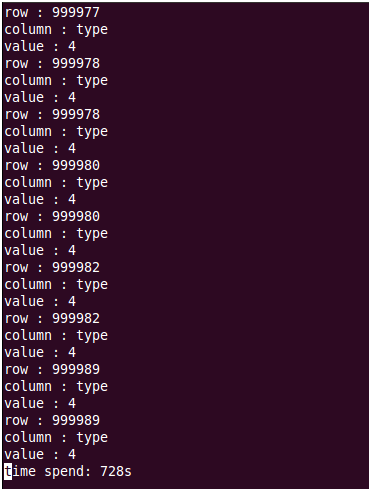
\includegraphics[scale=0.5]{photo/bcjg.png} 
\caption{mongoDB表的查询时间}
\end{figure} 